\begin{figure}[h] 
\centering 
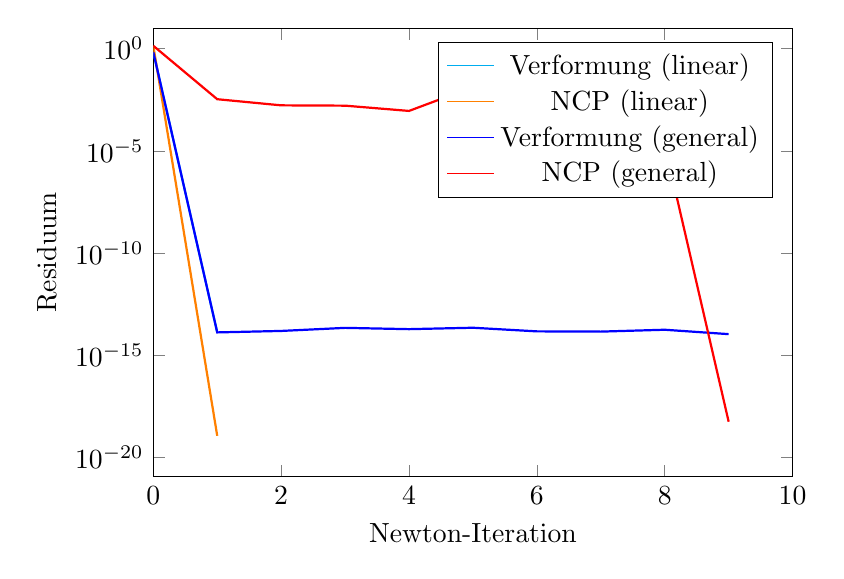
\begin{tikzpicture}[every plot/.append style={thick}] 
\begin{axis}[ 
label style={font=\normalsize}, 
xlabel={Newton-Iteration}, 
ylabel={Residuum}, 
xmin=0, xmax=10, 
ymode=log, 
ymin=0, ymax=10, 
width=0.8\textwidth, 
height=0.6\textwidth, 
legend pos=north east, 
legend style={cells={align=left}}, 
grid style=dashed, 
] 
\addplot[ 
color=cyan, 
] 
coordinates { 
(0, 6.82e-01)(1, 1.29e-14)}; 
\addlegendentry{Verformung (linear)} 
\addplot[ 
color=orange, 
] 
coordinates { 
(0, 1.38e+00)(1, 1.12e-19)}; 
\addlegendentry{NCP (linear)} 
\addplot[ 
color=blue, 
] 
coordinates { 
(0, 6.82e-01)(1, 1.29e-14)(2, 1.52e-14)(3, 2.15e-14)(4, 1.86e-14)(5, 2.18e-14)(6, 1.45e-14)(7, 1.41e-14)(8, 1.74e-14)(9, 1.06e-14)}; 
\addlegendentry{Verformung (general)} 
\addplot[ 
color=red, 
] 
coordinates { 
(0, 1.38e+00)(1, 3.35e-03)(2, 1.68e-03)(3, 1.62e-03)(4, 8.95e-04)(5, 1.33e-02)(6, 8.04e-04)(7, 7.83e-04)(8, 1.92e-05)(9, 5.47e-19)}; 
\addlegendentry{NCP (general)} 
\end{axis} 
\end{tikzpicture} 
\caption{Residuen des Stoffgesetzes 'Linear elastisch' mit Hinderniss 'Hut' und 2178 Freiheitsgraden für die Verschiebung.} 
\label{fiq:Linearelastisch_Hut_level4} 
\end{figure} 
